\documentclass[12pt,a4paper]{article}
\usepackage[utf8]{vietnam}
\usepackage{amsmath,amssymb}
\usepackage{tabularx}
\usepackage{tikz}
\usetikzlibrary{calc,angles,quotes,arrows.meta,patterns}
\usepackage{xcolor}
\usepackage{enumitem}
\usepackage{fancyhdr}
\usepackage[top=1.2cm, bottom=1.2cm, left=1.5cm, right=1.5cm]{geometry}
\usepackage[dethi]{ex_test}
\SAOPTN{widthSA=2.6,heightSA=0.62}

\setlength{\headheight}{15pt}
\setlength{\parskip}{0pt}

\pagestyle{fancy}
\fancyhf{}
\rhead{\textit{Môn Toán 6 -- Đề số 8}}
\lhead{\textit{Bộ đề ôn tập Giữa học kì I}}
\cfoot{\thepage}

\begin{document}

% --- KHUNG TIÊU ĐỀ ĐỀ THI ---
\noindent
\begin{tabularx}{\linewidth}{X r}
\textbf{TRƯỜNG THCS: \dotfill} & \textbf{ĐỀ KIỂM TRA ĐỊNH KỲ GIỮA HỌC KỲ I} \\
\textbf{Họ và tên: \dotfill} & \textbf{NĂM HỌC 2026 -- 2027} \\
\textbf{Lớp: \dotfill \quad SBD: \dotfill} & \textbf{Môn: TOÁN 6} \\
\hline
\end{tabularx}
\vspace{2mm}

\begin{center}
  \textbf{\large ĐỀ ÔN TẬP GIỮA HỌC KỲ I -- ĐỀ SỐ 8}\\
  \textit{Thời gian làm bài: 90 phút (Không kể thời gian phát đề)}
\end{center}
\vspace{1mm}

% --- PHẦN I ---
\noindent\textbf{\large PHẦN I. CÂU TRẮC NGHIỆM NHIỀU PHƯƠNG ÁN LỰA CHỌN (3,0 điểm)}

\textit{Thí sinh trả lời từ câu 1 đến câu 12. Mỗi câu hỏi thí sinh chỉ chọn một phương án duy nhất.}

\vspace{1mm}
\begin{ex}
Trong các số $23\,755; 10\,230; 17\,280; 18\,711$, số nào chia hết cho cả $2; 3; 5; 9$?
\choice
{$23\,755$}
{$10\,230$}
{\True $17\,280$}
{$18\,711$}
\end{ex}

\begin{ex}
Cho $A = \{x \in \mathbb{N}^* \mid x \le 12\}$. Tập hợp $A$ có số phần tử là:
\choice
{$10$}
{$11$}
{\True $12$}
{$13$}
\end{ex}

\begin{ex}
Cho $18 \ \vdots \ x$ và $7 \le x < 18$. Khi đó $x$ có giá trị là:
\choice
{$2$}
{$3$}
{$6$}
{\True $9$}
\end{ex}

\begin{ex}
Số nào sau đây không phải số nguyên tố?
\choice
{$11$}
{\True $33$}
{$17$}
{$31$}
\end{ex}

\begin{ex}
Phân tích số $40$ ra thừa số nguyên tố ta được kết quả đúng là:
\choice
{$2 \cdot 4 \cdot 5$}
{\True $2^3 \cdot 5$}
{$5 \cdot 8$}
{$4 \cdot 10$}
\end{ex}

\begin{ex}
Cho hình lục giác đều $ABCDEG$ tâm $O$. Khẳng định nào sau đây là đúng?
\begin{center}
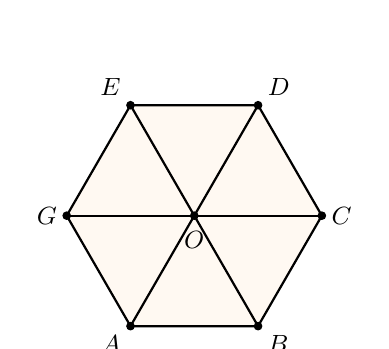
\begin{tikzpicture}[scale=0.9, font=\small]
  \coordinate (O) at (0,0);
  \foreach \i/\name in {0/C, 60/D, 120/E, 180/G, 240/A, 300/B} {
    \coordinate (\name) at (\i:1.8);
  }
  \draw[thick, fill=orange!5] (A) -- (B) -- (C) -- (D) -- (E) -- (G) -- cycle;
  \draw[thick] (A) -- (D);
  \draw[thick] (B) -- (E);
  \draw[thick] (C) -- (G);
  \filldraw (O) circle (1.5pt) node[below=2pt] {$O$};
  \filldraw (A) circle (1.5pt) node[below left] {$A$};
  \filldraw (B) circle (1.5pt) node[below right] {$B$};
  \filldraw (C) circle (1.5pt) node[right] {$C$};
  \filldraw (D) circle (1.5pt) node[above right] {$D$};
  \filldraw (E) circle (1.5pt) node[above left] {$E$};
  \filldraw (G) circle (1.5pt) node[left] {$G$};
\end{tikzpicture}
\end{center}
\choice
{\True $OA = OB = OC = OD = OE = OG$}
{$OA < OB < OC < OD < OE < OG$}
{$OA > OB > OC > OD > OE > OG$}
{$OA \ne OB \ne OC \ne OD \ne OE \ne OG$}
\end{ex}

\begin{ex}
Khẳng định nào sau đây là sai?
\choice
{Hình chữ nhật và hình thoi có các cặp cạnh đối song song với nhau}
{Hình lục giác đều có ba đường chéo chính bằng nhau}
{Hình bình hành có các cạnh đối bằng nhau}
{\True Hình thoi có hai đường chéo bằng nhau}
\end{ex}

\begin{ex}
Hình nào sau đây có tất cả các góc ở đỉnh bằng nhau?
\choice
{Hình thoi}
{\True Hình chữ nhật}
{Hình bình hành}
{Hình thang cân}
\end{ex}

\begin{ex}
Một hình thang cân có độ dài hai đáy là $a, b$ và chiều cao là $h$. Công thức tính diện tích hình thang đó là:
\choice
{\True $S = \dfrac{(a+b) \cdot h}{2}$}
{$S = \dfrac{(a-b) \cdot h}{2}$}
{$S = 2(a+b) \cdot h$}
{$S = \dfrac{a+b}{2} \cdot h^2$}
\end{ex}

\begin{ex}
Cho hình thoi $ABCD$, hai đường chéo $AC$ và $BD$ của hình thoi:
\choice
{Bằng nhau}
{Không vuông góc}
{\True Vuông góc với nhau}
{Cả A và B đều đúng}
\end{ex}

\begin{ex}
Viết gọn tích $8 \cdot 8 \cdot 2 \cdot 4$ dưới dạng lũy thừa cơ số 8 là:
\choice
{$8$}
{$8^2$}
{\True $8^3$}
{$8^4$}
\end{ex}

\begin{ex}
Một mảnh vườn hình chữ nhật có chiều dài $5\text{ m}$, chiều rộng $3\text{ m}$. Bác Bình muốn rào kín xung quanh mảnh vườn. Hỏi chiều dài hàng rào cần dùng là bao nhiêu mét?
\begin{center}
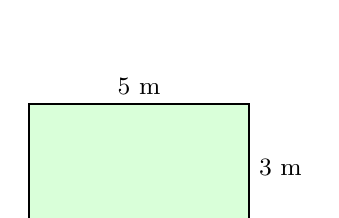
\begin{tikzpicture}[scale=0.8, font=\small]
  \coordinate (A) at (0,2);
  \coordinate (B) at (3.5,2);
  \coordinate (C) at (3.5,0);
  \coordinate (D) at (0,0);
  \draw[thick, fill=green!15] (A) -- (B) -- (C) -- (D) -- cycle;
  \node[above] at (1.75,2) {$5\text{ m}$};
  \node[right] at (3.5,1) {$3\text{ m}$};
\end{tikzpicture}
\end{center}
\choice
{\True $16\text{ m}$}
{$10\text{ m}$}
{$8\text{ m}$}
{$6\text{ m}$}
\end{ex}


\vspace{1mm}
\noindent\textbf{BẢNG TRẢ LỜI TRẮC NGHIỆM PHẦN I:}
\begin{center}
\begin{tabular}{|c|c|c|c|c|c|c|c|c|c|c|c|c|}
\hline
\textbf{Câu} & \textbf{1} & \textbf{2} & \textbf{3} & \textbf{4} & \textbf{5} & \textbf{6} & \textbf{7} & \textbf{8} & \textbf{9} & \textbf{10} & \textbf{11} & \textbf{12} \\
\hline
\textbf{Chọn} & \rule{0pt}{0.65cm} & & & & & & & & & & & \\
\hline
\end{tabular}
\end{center}
\vspace{2mm}

\setcounter{ex}{0}
\noindent\textbf{\large PHẦN II. CÂU TRẮC NGHIỆM ĐÚNG SAI (2,0 điểm)}

\textit{Thí sinh trả lời câu 1 và câu 2. Trong mỗi ý a), b), c), d) ở mỗi câu, thí sinh chọn đúng hoặc sai.}

\vspace{1mm}
\begin{ex}
Cho các hình sau: tam giác đều, hình vuông, lục giác đều, hình chữ nhật, hình thoi, hình bình hành, hình thang cân. Xét tính đúng/sai của các khẳng định sau:
\choiceTF
{\True Hình tam giác đều, hình vuông, hình lục giác đều có tất cả các cạnh bằng nhau}
{\True Có đúng 2 hình có hai đường chéo vuông góc với nhau}
{\True Có đúng 3 hình có các cạnh đối song song và hai đường chéo bằng nhau}
{Hình lục giác đều có độ dài mọi đường chéo đều gấp đôi độ dài cạnh}
\end{ex}

\begin{ex}
Một chiếc ô tô đang di chuyển với vận tốc ban đầu là $10\text{ km/h}$. Sau mỗi giờ, vận tốc tăng gấp đôi. Xét tính đúng/sai của các khẳng định sau:
\choiceTF
{\True Sau 1 giờ, vận tốc ô tô là $20\text{ km/h}$}
{Sau 2 giờ, vận tốc ô tô là $30\text{ km/h}$}
{\True Sau 3 giờ, vận tốc ô tô là $80\text{ km/h}$}
{\True Sau 4 giờ, vận tốc ô tô là $160\text{ km/h}$}
\end{ex}


\noindent\textbf{BẢNG TRẢ LỜI PHẦN II:}
\begin{center}
\begin{tabular}{|c|c|c|c|c||c|c|c|c|c|}
\hline
\textbf{Câu 1} & \textbf{a)} & \textbf{b)} & \textbf{c)} & \textbf{d)} & \textbf{Câu 2} & \textbf{a)} & \textbf{b)} & \textbf{c)} & \textbf{d)} \\
\hline
\textbf{Đ/S} & \rule{0pt}{0.6cm} & & & & \textbf{Đ/S} & & & & \\
\hline
\end{tabular}
\end{center}
\vspace{2mm}

\setcounter{ex}{0}
\noindent\textbf{\large PHẦN III. CÂU HỎI TRẢ LỜI NGẮN (2,0 điểm)}

\textit{Thí sinh trả lời câu 1 và câu 2. Điền kết quả số vào ô trống tương ứng.}

\vspace{1mm}
\begin{ex}
Có bao nhiêu số tự nhiên $m$ sao cho $5 < m < 10$ và $m$ chia hết cho 3? \shortans{2}
\end{ex}

\begin{ex}
Một hình chữ nhật có diện tích là $120\text{ cm}^2$ và có chiều dài là $12\text{ cm}$. Tính độ dài chiều rộng của hình chữ nhật đó (theo đơn vị $\text{cm}$). \shortans{10}
\end{ex}


\setcounter{ex}{0}
\noindent\textbf{\large PHẦN IV. TỰ LUẬN (3,0 điểm)}

\textit{Thí sinh trình bày chi tiết lời giải vào giấy làm bài.}

\vspace{1mm}
\begin{ex} (1,0 điểm)
Thực hiện phép tính (Tính nhanh nếu có thể):
\begin{enumerate}[label=\textbf{\alph*)}, leftmargin=0.8cm, itemsep=2pt]
\item (0,5 điểm) $127 + 156 + 73 + 144$
\item (0,5 điểm) $2026 - (20 \cdot 3^2 + 16 : 2^2)$
\end{enumerate}
\end{ex}
\vspace{1.5mm}

\begin{ex} (1,0 điểm)
Tìm số tự nhiên $x$, biết:
\begin{enumerate}[label=\textbf{\alph*)}, leftmargin=0.8cm, itemsep=2pt]
\item (0,5 điểm) $x - 18 = 15$
\item (0,5 điểm) $18 + 2(x - 1) = 40$
\end{enumerate}
\end{ex}
\vspace{1.5mm}

\begin{ex} (0,5 điểm)
Một hình chữ nhật có diện tích là $220\text{ cm}^2$ và có chiều dài là $22\text{ cm}$. Tính độ dài chiều rộng của hình chữ nhật (theo đơn vị $\text{cm}$).
\end{ex}
\vspace{1.5mm}

\begin{ex} (0,5 điểm)
Không thực hiện tính tổng, chứng minh rằng biểu thức sau chia hết cho 21:\\$A = 1 + 4 + 4^2 + 4^3 + \dots + 4^{2021}$
\end{ex}
\vspace{1.5mm}


\begin{center}
\rule{4cm}{0.4pt}\\
\textit{--- HẾT ---}
\end{center}
\end{document}
